\documentclass{article}
    \usepackage{xparse}
    \usepackage[margin=2cm]{geometry}
	\usepackage{enumerate} 
    \usepackage{textcomp}
	\frenchspacing
	\linespread{1.2}

    \usepackage[polish]{babel}
    \usepackage[utf8]{inputenc}
    \usepackage{polski}

	\usepackage{amsthm}
	\usepackage{amsmath}
	\usepackage{amsfonts}
	\usepackage{float}
    \usepackage{diagbox}
	\usepackage{hhline}
	\usepackage{graphicx}
	\usepackage{multirow}
	\usepackage{mathtools}

	\theoremstyle{definition}
	\newtheorem{zadanie}{Zadanie}[subsection]
	\renewcommand{\thezadanie}{\arabic{zadanie}}

\title{\textbf{Auxo: A Scalable and Efficient Graph Stream Summarization Structure\\
    Omówienie artykułu}}

\author{Paweł Polerowicz}
\date{Listopad 2023}

\begin{document}
    \maketitle
    \section{Wiadomości wstępne}
    
    \subsection{Informacje o artykule}
    \begin{itemize}
        \item Tytuł: Auxo: A Scalable and Efficient Graph Stream Summarization Structure
        \item Autorzy: Zhiguo Jiang, Hanhua Chen, Hai Jin
        \item Data publikacji: Luty 2023
        \item miejsce publikacji: Proceedings of the VLDB Endowment
    \end{itemize}
    
    \subsection{Słowniczek pojęć}

    \begin{tabular}{|l | l | } 
        \hline
        Oznaczenie & Znaczenie \\
        \hline\hline
        $G(V,E)$ & graf \\ 
        \hline
        $e_i = (<s_i,d_i>; w_i; t_i)$ & krawędź skierowana $s_i \rightarrow d_i$ z wagą $w_i$ i czasem pojawienia się $t_i$  \\ 
        \hline
        $f$ & długość podpisu \\ 
        \hline
        $b$ & rozmiar kubełka na zerowym poziomie \\ 
        \hline
        $h(v)$ & hash wierzchołka $v$ \\ 
        \hline
        $<\zeta_{s_i},\zeta_{d_i}>$ & podpis krawędzi $s_i \rightarrow d_i$ \\ 
        \hline
        $m$ & długość boku macierzy \\ 
        \hline
        $r$ & długość sekwencji hasha \\ 
        \hline
        $\{h_k(v)| 1 \leq k \leq r\}$ & sekwencja hasha \\ 
        \hline
        $p$ & liczba kubełkowych kandydatów \\ 
        \hline
        $l$ & liczba poziomów Auxo \\ 
        \hline
        $n$ & liczba zaalokowanych macierzy \\ 
        \hline
        $\alpha$ & stopień zapełnienia macierzy \\ 
        \hline
        $\zeta_{v}^{-i}$ & podpis wierzołka $v$ bez pierwszych $i$ bitów \\ 
        \hline
        $M_{l}^{x,y}$ & macierz przechowująca krawędzie z prefiksami podpisów $x, y$ na poziome $l$  \\ 
        \hline
    \end{tabular}\\
    
    \subsection{Plan prezentacji}
        W ramach niniejszej prezentacji zreferujemy artykuł \textit{Auxo: A Scalable and Efficient Graph Stream Summarization Structure}, przedstawiający strukturę Auxo. Jest to skalowalna struktura, wspierająca podsumowywanie strumieni grafów w efektywny czasowo i pamięciowo, przy zachowaniu wysokiej dokładności odpowiedzi na zapytania. Wykorzystuje ona drzewo prefixowe (PET), które wbudowuje prefiksy podpisów krawędzi w strukturę grafu. Dzięki temu czas wstawiania nowych krawędzi oraz wykonywania zapytań to $O(log|E|)$. Pokażemy również, że złożoność pamięciową możemy wyrazić jako $O(|E|(1 - log|E|))$. Auxo może także uzyskać lepsze wykorzystanie pamięci przez użycie proporcjonalnego PET.
    
    \section{Problem}
    
    \subsection{Sformułowanie problemu}
        Problemem, który staramy się rozwiązać jest znalezienie takiego sposobu przechowywania i analizy informacji o grafie, aby zminimalizować koszt pamięciowy w stosunku do tradycyjnych metod. Zależy nam także na uzyskaniu wysokiej efektywności czasowej dodawania nowych krawędzi oraz wykonywania zapytań. Zapytania dotyczą przede wszystkim kwestii istnienia oraz łącznej wagi krawędzi między dwoma wierzchołkami, ale także wagi krawędzi wchodzących i wychodzących z danego wierzchołka. Rozwiązania stratne są akceptowalne, jeśli oferują dobrą złożoność pamięciową i czasową. Dokładne wyniki i proporcje, które nas interesują są trudne do zdefiniowania. 
    
    \subsection{Główne idee rozwiązań}
        Większość istniejących rozwiązań problemu można podzielić na dwie grupy. Pierwsza z nich opiera się o MDL (Minimum description length). Metoda ta polega na znalezieniu dla zbioru danych $D$ modulu $M$ takiego, aby zminimalizować $L(M) + L(D|M)$, gdzie składniki sumy to odpowiednio długość danych potrzebnych do opisu $M$ oraz długość zakodowanego zbioru $D$. Są one skalowalne i w większości bezstratne, lecz nieefektywne dla wielkich i szybko zmieniających się grafów. Druga grupa to metody oparte o hasze. 

    \subsection{Poprzednie rozwiązania bazujące na haszach}
        \subsubsection{TCM}
            Najczęściej spotykanym podejściem jest w tym przypadku reprezentacja grafu w postaci skompresowanej macierzy haszy. Pierwszą próbą zastosowania tego pomysłu była struktura TCM. Używa ona funcji haszującej $h$, przyjmującą wartości ze zbioru $\{0, 1,\dots m - 1)$ (Na marginesie, a co, gdybyśmy użyli double i zakresów? Teoretycznie mniejsze ryzyko konfliktów - jeśli kubełek zajęty, to po prostu idziemy dalej. To trochę już załatwiają podpisy, więc może nieważne). Dla krawędzi $s_i \rightarrow d_i$, informacje o niej są przechowywane w komórce $M(h(s_i), h(d_i))$ macierzy. Zapytanie o pojedynczą krawędź jest oczywiste. In-flow/Out-flow liczymy, sumując odpowiednią kolumnę/wiersz. Ta struktura ma stały koszt pamięciowy i czasowy, ale jej oczywistym problemem jest brak skalowalności. Oznacza to, że dla większych grafów kolizje haszy mogą całkowicie wykluczyć pozyskiwanie wiarygodnych odpowiedzi na zapytania.
        
        \subsubsection{GSS}
            Ważną próbą odpowiedzi na słabości TCM była jego modyfikacja, nazwana GSS. Jej założeniem było przechowywania w komórkach macierzy nie tylko wag krawędzi, ale także podpisy wierzchołków wyznaczających daną krawędź. Pozwala to unikniecię konfliktów w przypadku konfliktu haszy. Gdy podczas wstawiania nowej krawędzi odpowiedni kubełek jest już zajęty, wykorzystywany jest oddzielny bufor. Autorzy proponują także metodę \textit{square hashing}, aby uzyskać więcej niż jeden kubełek kadydacki, a więc ograniczyć liczbę krawędzi w buforze. Niemniej jednak, wraz z rozmiarem grafu, coraz więcej krawędzi wyląduje w buforze, a złożoność pamięciowa wzrasta do liniowej względem liczby krawędzi. Pierwszym pomysłem na poprawę jest zastosowanie listy macierzy (GSS Chain). Po wypełnieniu jednej macirzy, alokowana jest kolejna. Łatwo jednak zauważyć, że nie rozwiązuje to problemu asymptotycznie liniowej złożoności pamięciowej.
            
    \section{Auxo}
    
    \subsection{Idea}
        Auxo czerpie inspiracje z klasycznych rozwiązań, wykorzystując macierze i funkcję haszującą. Ponadto zapożycza również podpisy krawędzi $<\zeta_{s_i},\zeta_{d_i}>$ znane z GSS. Jednak zamiast używać tylko jednej macierzy lub listy macierzy, Auxo wykorzystuje drzewo prefioksowe PET, którego wierzchołkami są takie własnie macierze. Dodatkowo, stara się ona ograniczyć wykorzystanie pamięci, poprzez zapisanie części informacji o podpisach w strukturze drzewa. 
    
    \subsection{Zasada działania}
        Zaczynamy z jedną macierzą o boku długości $m$. Jej elementami będą kubełki zawierające podpis krawędzi, łączną wagę oraz parę indeksów. Indeksy te są wyliczane na podstawie sekwencji haszy $\{h_k(v): 1 \leq k \leq r\}$, gdzie $r$ to niewielka stała. Mają one na celu zwiększenie gwarancji braku konfliktów. Wstawiając nową krawędź, generujemy wspomnianą sekwencję haszy wyzanczającą współrzędne $r^2$ kubełków, które sprawdzamy po kolei. Jeśli napotykamy kubełek pusty, wstawiamy tam informacje o krawędzi. Jeśli kubełek nie jest pusty, sprawdzamy podpisy i indeksy. Jeśli się zgadzają, akumulujemy wagę krawędzi. Jeśli nie byliśmy w stanie wstawić krawędzi, przechodzimy do następnej macierzy zgodnie ze strukturą drzewa, lub, jeśli jesteśmy w liściu, tworzymy nowy poziom drzewa. Możemy stosować drzewo binarne, wbudowując na zmianę prefiks z jednego lub drugiego hasza, lub 4-arne, używając obu naraz. W praktyce ograniczymy się do binarnego.
    \subsection{Przykład}
        Rozważmy drzewo o dwóch pozionach, jak poniżej. Załóżmy, że otrzymujemy krawędź $s_i \rightarrow d_i$ o podpisie $<\zeta_{s_i},\zeta_{d_i}> = <101, 110>$. Załóżmy, że kubełki w $M_0$ są już zajęte i sprawdzamy $M_0^{\emptyset, 1}$ jak na drugim rysunku. Obliczamy sekwencje haszy $hq_{s_i} = \{0, 2\}, hq_{d_i} = \{0, 3\}$. Sprawdzamy najpierw $M_0^{\emptyset, 1}[0,0]$, ale jest już zajęty i podpisy się nie zgadzają. Natomiast w przypadku $M_0^{\emptyset, 1}[2,3]$ wszystko się zgadza, więc aktualizujemy wagę krawędzi. W przypadku, gdyby komórka była pusta, po prostu wstawilibyśmy do niej kubełek z informacjami o nowej krawędzi. 
    \begin{figure}[H]
        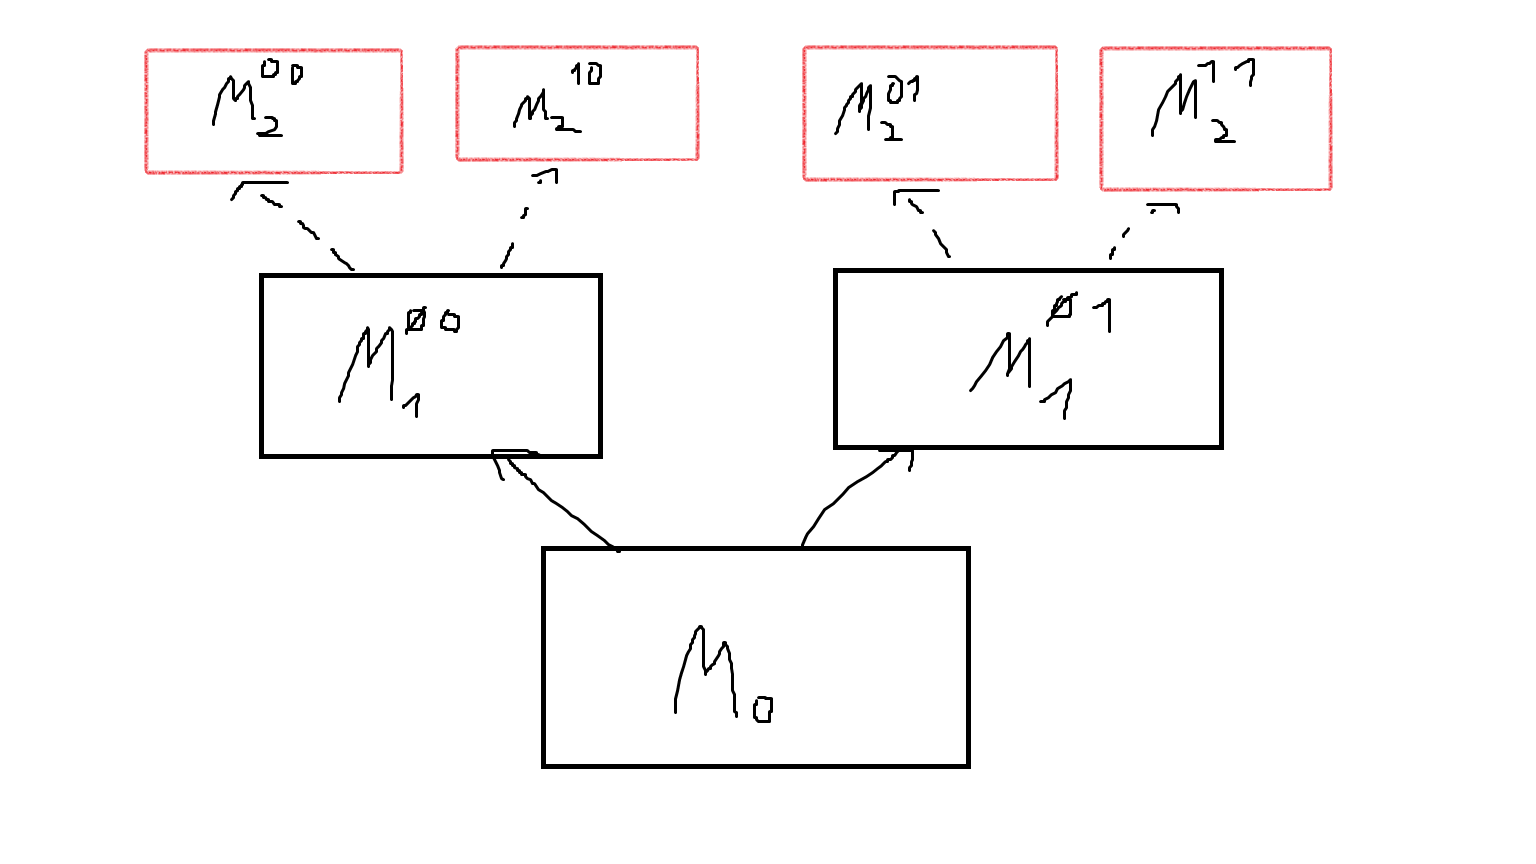
\includegraphics[width=11cm]{img/Auxo1.png}
        \centering
    \end{figure}
        \begin{figure}[H]
        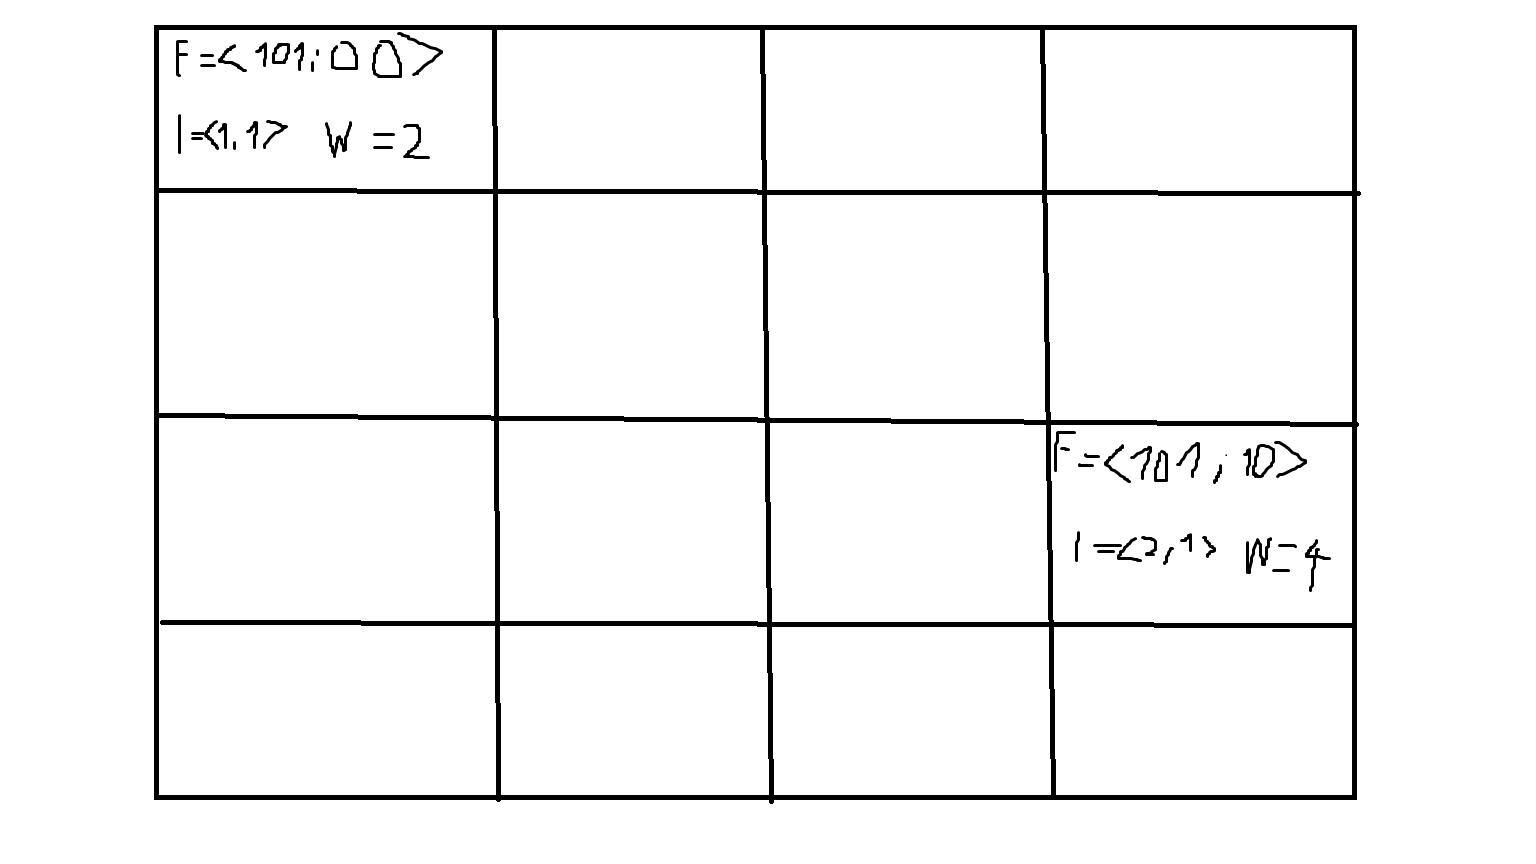
\includegraphics[width=11cm]{img/Auxo2.png}
        \centering
    \end{figure}

    \subsection{Proporcjonalny przyrost drzewa}
        Aby zapewnić równomierny przyrost drzewa i efektywne wykorzystanie pamięci, możemy wykorzystać pomocniczą strukturę \textit{Deputy tree}. Nowe krawędzie, jeśli nie mogą zostać wstawione do głównego drzewa, są wstawiane do \textit{Deputy tree}. Przypomina ono drzewo główne, z tą róznicą, że ma tylko jeden poziom. Gdy zachodzi potrzeba stworzenia kolejnego, krawędzie z obecnego poziomu są przepisywane do nowych macierzy, aż skontruowany zostanie nowy poziom głównego drzewa.
    
    \subsection{Złożoność pamięciowa}
    Złożoność pamięciowa jest prosta do wyznaczenia. Załóżmy, że drzewo PET w Auxo ma $l$ poziomów. Wtedy ilość zaalokowanej pamięci możemy wyrazić jako:
    \[
        M_A = m^2 b (2^l - 1) - \sum_{i=0}^{l-1}m^2 i 2^i = m^2(b(2^l - 1) - 2^l(l - 2) - 2)
    \]
    Pierwszy składnik sumy można potraktować jako łączny rozmiar wszystkich macierzy przy założeniu, że rozmiar kubełków na każdym poziomie jest jednakowy. Wtedy rzeczywiście, w pojedynczej macierzy mamy $m^2$ kubełków o rozmiarze b, a całe drzewo ma łącznie $2^l - 1$ takich macierzy. Oczywiście, w rzeczywistości rozmiar kubełków maleje o 1 na każdym poziomie, co odzwierciedla odejmowana suma. Na poziomie $i$ mamy $2^i$ macierzy po $m^2$ kubełków i w każdym z nich oszczędzamy $i$ bitów. W obliczeniach pomijamy pamięć zaalokowaną na potrzeby \textit{Deputy tree}, jednak łatwo zauważyć, że nie przekracza ona $m^2 b 2^l$, więc nie wpływa na asymptotykę złożoności. Moglibyśmy równoważnie powiedzieć, że powyższy wzór dotyczy głównego drzewa o $l - 1$ poziomach z uwzględnieniem \textit{Deputy tree}.

    Podstawiając $l = log_2\frac{|E|}{m^2\alpha}$ otrzynujemy złożoność $O(|E|(1 - log|E|))$. Wynik ten może wywoływać dyskomfort wsród czytelników, gdyż bez odpowiedniej interpretacji, może on sugerować ujemną złożoność dla większych struktur. Zauważmy jednak, całościowy rozmiar struktury jest ograniczony przez liczbę bitów $b$ kubełka. Oczywiście, rozmiary kubełków nie mogą być ujemne, a w praktyce nie mogą nawet być mniejsze niż pewna wartość $b_{min}$ potrzebna do przechowywania wagi krawędzi. Po osiągnięciu tego momentu moglibyśmy dalej rozszerzać drzewo, doczepiając już tylko po jednym synie do liści, ale to dałoby nam ostatecznie liniową złożoność czasowa W takim przypadku należałoby raczej zastonowić na zwiększeniem długości podpisów, a więc i $b$. W praktyce jednak nawet stosunkowo niewielkie długości podpisów gwarantują dużą liczbę możliwych do przeprocesowania krawędzi.
    
    \subsection{Złożoność czasowa (szkic)}
        Złożoność czasowa zapytania o wagę krawędzi jest naturalnie naturalnie logarytmiczna. Na każdym poziomie struktury sprawdzamy tylko jedną macierz i w każdej macierzy sprawdzamy co najwyżej r kubełków. W przypadku wstawiania krawędzi, procedura wygląda podobnie. Należy jednak zastanowić się nad momentem rozszerzania struktury o nowy poziom. Rozważmy wersję proporcjonalną i konstruowanie l-tego poziomu. Będzie to czas zamortyzowany. Oznaczmy czas przeszukiwania pojedynczej macierzy jako $\tau$ i czas przepinania krawędzi jako $\iota (\iota << \tau)$. Zakładamy, że macierz zawiera średnio $a_n$ krawędzi. Koszt wstawiania krawędzi 
        \[
            IT_l \leq (n_al\tau + n_al\tau + 2n_al\tau + \dots + 2^{l-2}n_al\tau) = 2^{l-1}n_al\tau
        \]
        Koszt przpinania krawędzi \textit{Deputy Tree} 
        \[
            MT_l \leq (n_a\iota + 2n_a\iota + \dots + 2^{l-2}n_a\iota) = (2^{l-1} - 1)n_a\iota
        \]
        Wtedy koszt zamortyzowany możemy zapisać jako
        \[
            AT_l = \frac{(MT_l + IT_l)}{2^{l-1}n_a} \leq l\tau + \frac{(2^{l-1} - 1)\iota}{2^{l-1}}
        \]
        Oczywiście $AT_l = O(l\tau) = O(log|E|)$.
        
    
    \subsection{Dokładność}
        Auxo zapewnie spełnienie:
        \[
            Pr((\hat{f}(s,d) - f(s,d)) / \bar{w} > \sigma) \leq \frac{|E|}{\sigma m^2 4^f}
        \]
        gdzie $\hat{f}(s,d)$ to odpowiedź, $f(s,d)$ to prawdziwa wartość, $\bar{w}$ to średni koszt krawędzi, a $f$ to długość podpisu. Dowód z Markova, ale skomplikowany i odwałuje się do innej pracy.
    
    \section{Zakończenie}
    Dziękuję słuchaczom za uwagę i życzę miłego dnia. 
    
\end{document}